\section{Case Studies}
\label{sec:casestudy}
The following text describes two real-world scenarios for \AVOIRmethodname{}. 
We implement Verifair inference rules in the \AVOIRmethodname{} (denoted as \AVOIRmethodname{}-VF) framework, which allows us to sidestep the assumptions of a having a known data generating distribution, making it more efficient than Verifair.
\todo{Explaining \AVOIRmethodname{}-VF}
We denote \AVOIRmethodname{}-OB as the implementation which also utilizes the constraints and optimization framework.
An important case study on the COMPAS dataset can be found in Appendix~\ref{sec:appendix:additional-case-studies}. 
\subsection{Rate My Profs}
\label{sec:casestudy:rmp}
%\pmcomment{SP: I think it would be good to include the Adult results here if there is space at least in as far as the effectiveness of the optimization to match Figure 4. Once you've finalized other sections we can look at space.}
In this section, we provide a detailed black-box machine learning model (ML) based case study on a real-world dataset.
%Table~\ref{tab:casestudy:summary} summarizes the results from the three studies.
%\pmcomment{Call out - name of DB, materialized view etc details}
In this case study, we use the rate my professors (RMP) dataset released by \citet{keymanesh2021fairness}. 
This dataset includes professor names and reviews for them written by students in their classes, ratings, and certain self-reported attributes of the reviewer.
Ratings are provided on a five-point scale (1-5 stars).
We use the preprocessing described in~\citet{keymanesh2021fairness} to infer the gender attribute for the professors.
This dataset is divided into an 80-20 split (train-test).
We then train a BERT-based transformer model~\cite{devlin2019bert} on the training split.
We use the implementation from the simpletransformers\footnote{https://simpletransformers.ai/} package.
The loss function chosen is the mean-squared error from the true ratings.
On the test set, we track a gender-fairness specification in the model outputs:
\begin{lstlisting}[columns=flexible, language=Python]
(E[r > 3 | gender = F] / E[r > 3 | gender = M < 1.2) & 
(E[r > 3 | gender = M)] / E[r > 3 | gender = F] > 0.8)
\end{lstlisting}
We set the failure probability $\Delta = 0.05$. 
\texttt{OPT} is run after each batch (5 items/batch).
Figure~\ref{fig:casestudy:rmp} shows that \AVOIRmethodname{}-OB\footnote{OB = Optimized Bounds} can provide a guarantee in $\mathbf{2.5\%}$ fewer iterations than \AVOIRmethodname{}-VF. 
Note also that the OB guarantee provided tries to optimize for the failure probability while staying under the required threshold, remaining closer to the required threshold in subsequent steps.

\subsection{Adult Income}
\label{sec:casestudy:adult}
%\pmcomment{TODO: Add visualization of tree, and ref further discussion in appendix. 
 %   \\ SP: For all graphs please uniformly refer to AVOIR-OB - AVOIR Optimized Bounds and AVOIR-VF - AVOIR VeriFair bounds instead of ours and VeriFair. Important to assert that AVOIR is the framework that allows you to compare these visually and empirically.}

In this case study we use the Adult income dataset~\citep{kohavi1996scaling} which has been used frequently in prior fairness-related work.
The historical dataset labels individuals from the 1994 census as having a \emph{high-income} ($>50,000$ a year) or not ($\leq50,000$ a year).
%\pmcomment{Reference interactive edits for updates}
%We consider a decision tree classifier that predicts if an individual has a high income.
%We leave 1,200 data points out as our test set and train on the rest.
In this case study, we look at a column of data as a black-box measurement (internally, we use a materialized view, details in Appendix~\ref{sec:appendix:additional-case-studies:materialized-view}).


US Federal laws mandate against race and sex based discrimination.
Thus, the specification we start our analysis with is a group fairness property that monitors the difference of the proportions of individuals with sex recorded as male that have a high income to females that have a high income should be less than $0.5$. In addition, we ensure that the difference between individuals with race marked as white and those without should have a difference of less than $0.5$.  
The associated specification is given below, where \texttt{h} is an indicator for whether an individual is \emph{high-income} is the binary classification output of our model:

\begin{lstlisting}[columns=flexible, language=Python]
   (E[h | sex=M] - E[h | sex=F] < 0.5) & \ 
   (E[h | race=W] - E[h | race!=W] < 0.5)
\end{lstlisting}

In this example, we set the failure threshold probability $\Delta = 0.15$
%, i.e., the assertion should be guaranteed with less than $15\%$ probability of failure.

\begin{figure}[ht]
    \centering
    \begin{subfigure}{0.48\linewidth}
    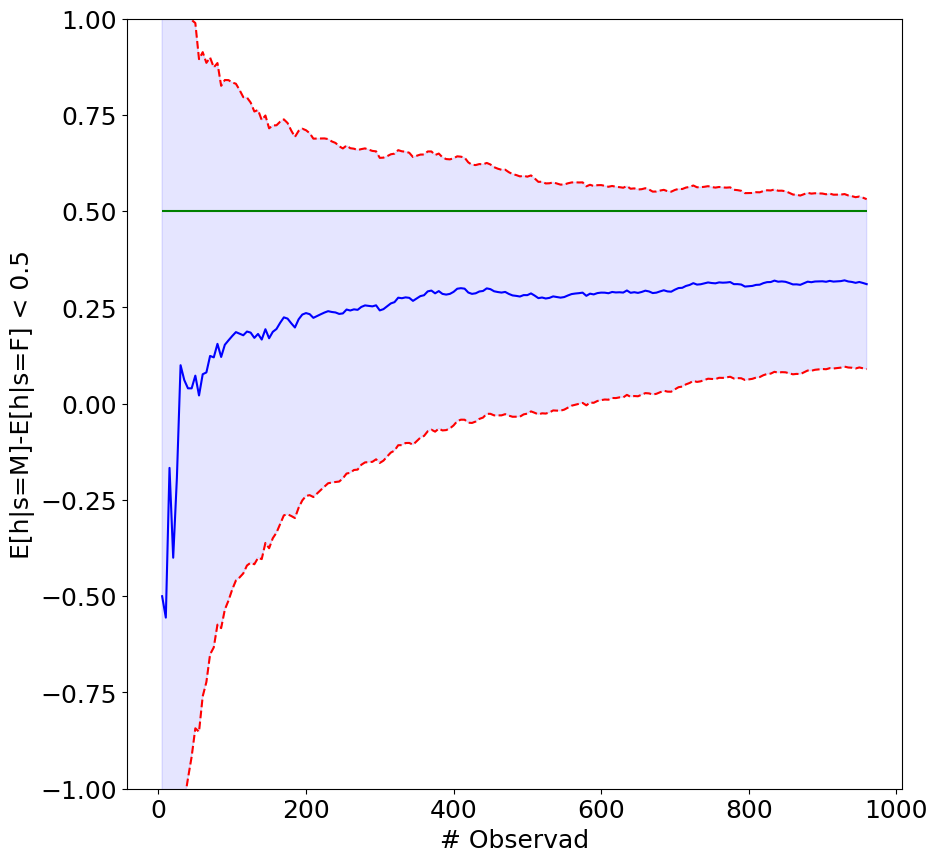
\includegraphics[width=\linewidth]{avoir/images/adult-left-initial.png}
    \caption{Group fairness for sex. Difference in ratio of high income earners in left subtree for initial specification.}
    \label{fig:casestudy:adult:specplot:left}
    \end{subfigure}
    \hfill
    \begin{subfigure}{0.48\linewidth}
    \centering
    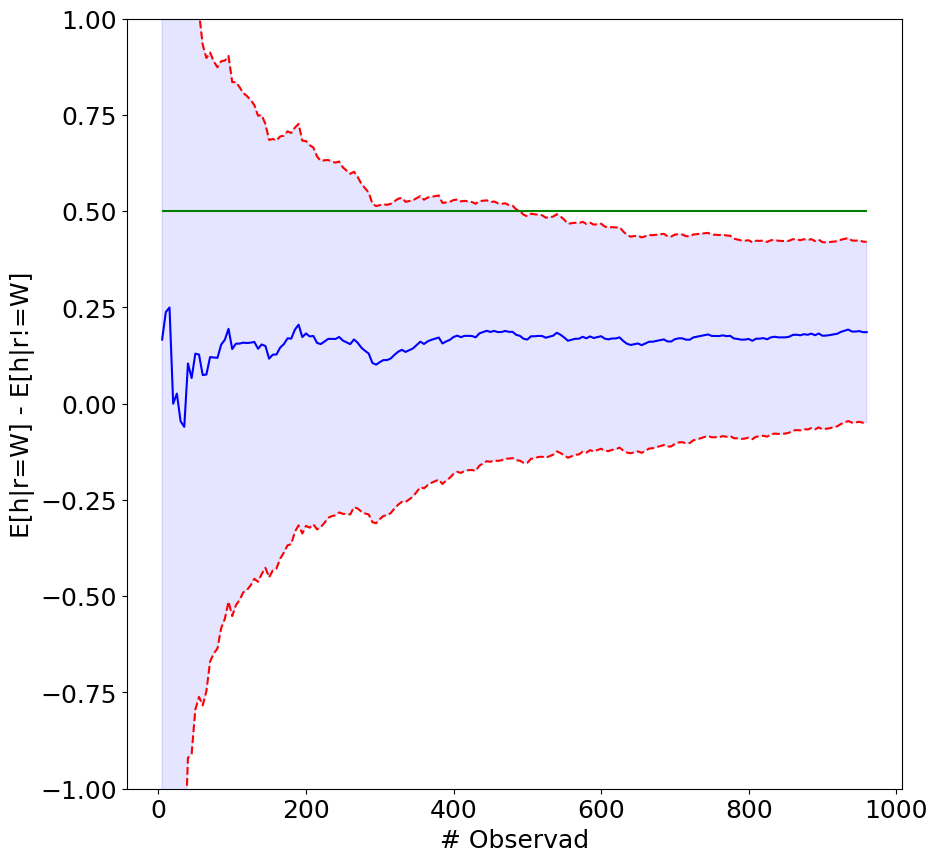
\includegraphics[width=\linewidth]{avoir/images/adult-right-initial.png}
    \caption{Group fairness for race (difference in ratio of high income earners) in right subtree for initial specification.}
    \label{fig:casestudy:adult:specplot:right}
    \end{subfigure}
    \caption{\figleft{}  Red dotted lines the upper bound of the value cannot be guaranteed to be under the threshold at the specified failure probability. \figright{} Guarantee possible with given data.}
\end{figure}


When run with this specification, the generated materialized view cannot achieve the required bound. 
We can then use our iterative refinement visualization tool to analyze different components of the specification. 
A developer would first interact with the left subtree of the specification. 
Due to paucity of space, this visualization is presented in Appendix~\ref{sec:appendix:additional-case-studies:viz}.
The plot for the corresponding data is shown in Figure~\ref{fig:casestudy:adult:specplot:left} shows that guarantees cannot converge under the threshold with the given number of data samples. 
The developer can now choose to either reduce the guarantee (i.e. reduce $\delta$) or increase the threshold. 
Next, analyzing the right subtree, the race group fairness term can be guaranteed to be under the threshold (Figure~\ref{fig:casestudy:adult:specplot:right}).
Using this information, the developer can make an intelligent decision to increase the threshold on the group fairness for term for sex. 
Suppose they increase it to $0.55$ and rerun the analysis.
OB is able provide a guarantee at this threshold within 870 steps, whereas VF can provide it at 960 steps, demonstrating a relative improvement of about $\mathbf{10.35\%}$.
Additionally, the optimal $\delta$ split across the terms are $\approx (0.135, 0.36 * 10^4)$ which is far from the equal split allocated by VF.
The reason for this split is because increasing the threshold for the first time provides the optimizer with additional legroom to better distribute the failure probabilities between the two terms.
%Further details, including a case study on the COMPAS dataset, are provided in Appendix~\ref{sec:appendix:additional-case-studies}.
%\pmcomment{Another potential addition is the distribution of $\delta$ across the terms - deltas are $(0.13476892449046354, 0.0003603486601995523)$ with optimization allocating a majority of the $delta$ to the first term. TODO Add - I think this will be a good addition - SP.}
%\pmcomment{Add summary table to case study}
%\pmcomment{
%\begin{itemize}
%    \item Model: Transformer, predict ratings from comments only.
%    \item Spec: 20\% rule for high ratings across genders
%    \item Our approach can achieve optimality sooner (2360 vs 2420 observations)
%\end{itemize}}